%--------------------------------------------------------------------------
% @file informe_tp1.tex
%
% @date 10/25/16 19:53:28
% @author Martin Noblia
% @email mnoblia@disroot.org
%
% @brief
%
% @detail
%
% Licence:
%This program is free software: you can redistribute it and/or modify
%it under the terms of the GNU General Public License as published by
%the Free Software Foundation, either version 3 of the License, or (at
%your option) any later version.
%
%This program is distributed in the hope that it will be useful, but
%WITHOUT ANY WARRANTY; without even the implied warranty of
%MERCHANTABILITY or FITNESS FOR A PARTICULAR PURPOSE.  See the GNU
%General Public License for more details.
%
%You should have received a copy of the GNU General Public License
%---------------------------------------------------------------------------
% Start
%---------------------------------------------------------------------------
\documentclass[10pt]{article}
%---------------------------------------------------------------------------
% Packages
%---------------------------------------------------------------------------
\usepackage{amsmath, siunitx}
\usepackage[table,xcdraw]{xcolor}
\usepackage{tikz}
\usepackage{epigraph}
\usepackage{lipsum}
\usepackage[colorlinks]{hyperref}
\usepackage{listings}
\usepackage{fancyhdr}
\usepackage[utf8]{inputenc}
\usepackage{hyperref}
\usepackage[spanish]{babel}
\usepackage{amsmath}
\usepackage{amsthm}
\usepackage{amssymb}
\usepackage{latexsym}
% \usepackage{graphicx}
\usepackage{color}
\usepackage{moredefs}
\usepackage{fancybox}
\usepackage{subfig}
\usepackage{float}
\usepackage{wallpaper}
\usepackage{textcomp}
\usepackage{minted} % for syntax highlight
\usepackage{textcomp} % for the TradeMark shit
\usepackage{enumerate}
\usepackage{cite}
\usepackage{minted} % for syntax highlight
\usepackage{circuitikz} % for the electric circuit
\usepackage{gensymb}
\usetikzlibrary{arrows}
\usetikzlibrary{bending}
\usetikzlibrary{babel}
%---------------------------------------------------------------------------
% Definitions
%---------------------------------------------------------------------------
\oddsidemargin -0.2in \textwidth 7.0in \topmargin -0.9in \textheight
9.0in
\parindent 3em
%---------------------------------------------------------------------------
% Cut of Spanish words
%---------------------------------------------------------------------------
\hyphenation{e-jem-plo
e-rro-res de-pen-dien-te co-rrien-te res-pues-ta fi-gu-ran
cons-tan-tes o-pe-ra-cion i-lu-mi-na-cion}
%---------------------------------------------------------------------------
% Colors
%---------------------------------------------------------------------------
\definecolor{azul-claro}{rgb}{0.335,0.89,1}
\definecolor{gainsboro}{rgb}{0.86,0.86,0.86}
\definecolor{mediumseagreen}{rgb}{0.24,0.7,0.44}
\definecolor{moccasin}{rgb}{1,0.89,0.71}
\definecolor{cornflowerblue}{rgb}{0.39,0.58,0.93}
\definecolor{lightgray}{rgb}{0.83,0.83,0.83}
\definecolor{darkgrey}{rgb}{0.66,0.66,0.66}
\definecolor{darkslategray}{rgb}{0.18,0.31,0.31}
\definecolor{lavender}{rgb}{0.9,0.9,0.98}
\definecolor{azure}{rgb}{0.94,1,1}
\definecolor{honeydew}{rgb}{0.94,1,0.94}
%---------------------------------------------------------------------------
% Page styles
%---------------------------------------------------------------------------
\renewcommand{\headrulewidth}{1pt}% 2pt header rule
\renewcommand{\headrule}{\hbox to\headwidth{%
\color{lightgray}\leaders\hrule height \headrulewidth\hfill}}

\pagestyle{fancy}
\headheight 50pt
\renewcommand{\arrayrulewidth}{3pt}
\newtheorem{defi}{{\it Definición}}[section]
%---------------------------------------------------------------------------
% Header page
%---------------------------------------------------------------------------
\rhead{
\includegraphics[width=.075\textwidth]{./Images/logo_iaci2.eps}} % iaci logo
\chead{}
\lhead{Procesos y Máquinas 2}
\rfoot{2º cuatrimestre 2017  }
\cfoot{\thepage}
\lfoot{\bf{Universidad Nacional de Quilmes}}
%---------------------------------------------------------------------------
% Custom section header(this shit generate a box color)
%---------------------------------------------------------------------------
\renewcommand{\arrayrulewidth}{1pt}
\newcommand{\mcaja}[1]{%
{{\fboxsep 12pt \fboxrule 2pt%
\fcolorbox{black}{darkgrey}{%
\color{red} \Huge #1}}}
}
\newcommand{\nuevobox}[1]{%
{{\fboxsep 14pt \fboxrule 1pt%
\fcolorbox{black}{darkgrey}{%
\color{lavender} \huge #1}}}
}
\newcommand{\ssection}[1]{\section[#1]{\mcaja{#1}}}
\makeatletter
\newcommand{\sect}[1]{\subsection[#1]{\nuevobox{#1}}}
\makeatletter
\def\section{\@ifstar\unnumberedsection\numberedsection}
\def\numberedsection{\@ifnextchar[%]
\numberedsectionwithtwoarguments\numberedsectionwithoneargument}
\def\unnumberedsection{\@ifnextchar[%]
\unnumberedsectionwithtwoarguments\unnumberedsectionwithoneargument}
\def\numberedsectionwithoneargument#1{\numberedsectionwithtwoarguments[#1]{#1}}
\def\unnumberedsectionwithoneargument#1{\unnumberedsectionwithtwoarguments[#1]{#1}}
\def\numberedsectionwithtwoarguments[#1]#2{%
\ifhmode\par\fi
\removelastskip
\vskip 3ex\goodbreak
\refstepcounter{section}%
\begingroup
%\noindent
\leavevmode\large\bfseries\raggedright\mcaja%%
\thesection\ #2\par\nobreak
\endgroup
\noindent\hrulefill\nobreak
\vskip 2ex\nobreak
\addcontentsline{toc}{section}{%
\protect\numberline{\thesection}%
#1}%
}
\def\unnumberedsectionwithtwoarguments[#1]#2{%
\ifhmode\par\fi
\removelastskip
\vskip 3ex\goodbreak
% \refstepcounter{section}%
\begingroup
\noindent
\leavevmode\Large\bfseries\raggedright
% \thesection\
#2\par\nobreak
\endgroup
\noindent\hrulefill\nobreak
\vskip 0ex\nobreak
\addcontentsline{toc}{section}{%
%
\protect\numberline{\thesection}%
#1}%
}
\makeatother
%%%Cap\’itulos
\usepackage{helvet}
%\usepackage{psboxit,pstcol}
\makeatletter
\def\@makechapterhead#1{%
{\parindent \z@ \raggedright \reset@font
\hbox to \hsize{%
\rlap{\raisebox{-2.5em}{\raisebox{\depth}{%%% Necesita la imagen "imgCapitulo"

\includegraphics[width=10em]{./Images/logo_iaci2.eps}}}}%
\rlap{\hbox to 6em{\hss
\reset@font\sffamily\fontsize{8em}{8em}\selectfont\black
\thechapter\hss}}%
\hspace{10em}%
\vbox{%
\advance\hsize by -10em
\reset@font\fontfamily{hv}\bfseries\Large
#1
\par
}%
}}%
\vskip 5pt
\hrulefill
\vskip 50pt
}
%---------------------------------------------------------------------------
% Redefinition of Theorems and Corollarys
%---------------------------------------------------------------------------
\makeatother
\newtheorem{theorem}{Teorema}[section]
\newtheorem{corollary}{Corolario}[theorem]
\newtheorem{lemma}[theorem]{Lema}
%---------------------------------------------------------------------------
% Title Page decoration
%---------------------------------------------------------------------------
\definecolor{titlepagecolor}{cmyk}{.73,.37,0,.37}


\newcommand\titlepagedecoration{%
\begin{tikzpicture}[remember picture,overlay,shorten >= -10pt]

\coordinate (aux1) at ([yshift=-15pt]current page.north east);
\coordinate (aux2) at ([yshift=-410pt]current page.north east);
\coordinate (aux3) at ([xshift=-4.5cm]current page.north east);
\coordinate (aux4) at ([yshift=-150pt]current page.north east);

\begin{scope}[titlepagecolor!40,line width=12pt,rounded corners=12pt]
\draw
  (aux1) -- coordinate (a)
  ++(225:5) --
  ++(-45:5.1) coordinate (b);
\draw[shorten <= -10pt]
  (aux3) --
  (a) --
  (aux1);
\draw[opacity=0.6,titlepagecolor,shorten <= -10pt]
  (b) --
  ++(225:2.2) --
  ++(-45:2.2);
\end{scope}
\draw[titlepagecolor,line width=8pt,rounded corners=8pt,shorten <= -10pt]
  (aux4) --
  ++(225:0.8) --
  ++(-45:0.8);
\begin{scope}[titlepagecolor!70,line width=6pt,rounded corners=8pt]
\draw[shorten <= -10pt]
  (aux2) --
  ++(225:3) coordinate[pos=0.45] (c) --
  ++(-45:3.1);
\draw
  (aux2) --
  (c) --
  ++(135:2.5) --
  ++(45:2.5) --
  ++(-45:2.5) coordinate[pos=0.3] (d);
\draw
  (d) -- +(45:1);
\end{scope}
\end{tikzpicture}%
}


\newcommand*{\plogo}{\fbox{$\mathcal{PL}$}}
\newcommand*{\titleGP}{\begingroup % Create the command for including the title page in the document
\centering % Center all text
\vspace*{\baselineskip} % White space at the top of the page

\rule{\textwidth}{1.6pt}\vspace*{-\baselineskip}\vspace*{2pt} % Thick horizontal line
\rule{\textwidth}{0.4pt}\\[\baselineskip] % Thin horizontal line

{\LARGE Procesos y Máquinas industriales 2\\[0.3\baselineskip] \textit{Trabajo Práctico Obligatorio}}\\[0.2\baselineskip] % Title

\rule{\textwidth}{0.4pt}\vspace*{-\baselineskip}\vspace{3.2pt} % Thin horizontal line
\rule{\textwidth}{1.6pt}\\[\baselineskip] % Thick horizontal line

\scshape % Small caps
{\Large Martín Noblía\\}
\vspace*{2\baselineskip} % Whitespace between location/year and editors

Profesora: \\[\baselineskip]
{\Large Mariana Suarez\\}
\vspace*{2\baselineskip} % Whitespace between location/year and editors
Instructor: \\[\baselineskip]
{\Large Roberto Peyton\\}
\vfill % Whitespace between editor names and publisher logo_iaci2

\includegraphics[width=.175\textwidth]{./Images/logo_iaci2.eps}

% Editor list
{\itshape Universidad Nacional de Quilmes \par} % Editor affiliation

\vfill % Whitespace between editor names and publisher logo

%\plogo \\[0.3\baselineskip] % Publisher logo
{\scshape 2017} \\[0.3\baselineskip] % Year published
%{\large THE PUBLISHER}\par % Publisher

\endgroup}
%---------------------------------------------------------------------------
% Begin of the document
%---------------------------------------------------------------------------
\begin{document}
\pagestyle{empty}

\titleGP
\titlepagedecoration

\newpage
\pagestyle{fancy}
\section{Modelado y simulación de un sistema térmico por analogía con un circuito eléctrico}
\subsection{Diseño y modelización} \label{modelado}
\begin{enumerate}
   \item Utilizando la analogía de los sistemas eléctricos, modelar matemáticamente el sistema correspondiente al circuito mostrado en la figura 1, que representa un dispositivo electrónico de potencia sin disipador.
   \item En la práctica y para poder garantizar condiciones operativas seguras se utilizan disipadores, tal como se plantea en la introducción. Desarrollar el circuito térmico equivalente para un dispositivo electrónico de potencia con disipador. Identificar en forma clara el circuito implementado y modelar matemáticamente el sistema propuesto.
\end{enumerate}
\subsubsection{Resolución}
Los circuitos eléctricos pueden utilizarse para modelar problemas de conducción de calor. Esta analogía consiste en tratar a la temperatura
como si fueran diferencias de potencial eléctrico, a los flujos de calor como corrientes, a los diferentes modos de transferencia de calor
como resistencias y a los fenómenos de almacenamiento de calor como capacitores. La siguiente tabla resume estas equivalencias:
%------------------------------------------------------------------------------
%                      tabla analogias
%------------------------------------------------------------------------------
\begin{table}[H]
\centering
\caption{Analogías entre los modelos electrico y térmico}
\label{tabla:analogias}
\begin{tabular}{|
>{\columncolor[HTML]{ECF4FF}}l |c|c|
>{\columncolor[HTML]{9AFF99}}l |c|c|}
\hline
\multicolumn{3}{|c|}{\cellcolor[HTML]{EFEFEF}\textbf{Modelo térmico}}                                                                                                            & \multicolumn{3}{c|}{\cellcolor[HTML]{EFEFEF}{\color[HTML]{000000} \textbf{Modelo eléctrico}}}                                                                                   \\ \hline
\multicolumn{1}{|c|}{\cellcolor[HTML]{9B9B9B}\textit{\textbf{variable}}} & \cellcolor[HTML]{9B9B9B}\textit{\textbf{simbolo}} & \cellcolor[HTML]{9B9B9B}\textit{\textbf{unidades}} & \multicolumn{1}{c|}{\cellcolor[HTML]{9B9B9B}\textit{\textbf{variable}}} & \cellcolor[HTML]{9B9B9B}\textit{\textbf{simbolo}} & \cellcolor[HTML]{9B9B9B}\textit{\textbf{unidades}} \\ \hline
Temperatura                                                              & $T$                                                 & $^{\circ}C$                                      & $\Delta E$                                                              & $V$                                                 & Volts                                            \\ \hline
Flujo de calor                                                           & $q$                                                 & $W$                                              & Corriente                                                               & $i$                                                 & Amperes                                          \\ \hline
Resistencia Térmica                                                      & $R$                                                 & $^{\circ}C / cal$                                & Resistencia                                                             & $R$                                                 & Ohms                                              \\ \hline
Capacidad térmica                                                        & $C$                                                 & $cal / ^{\circ}C$                                & Capacitancia                                                            & $C$                                                 & Faradays                                          \\ \hline
\end{tabular}
\end{table}
%------------------------------------------------------------------------------
%                      fin tabla analogias
%------------------------------------------------------------------------------
%------------------------------------------------------------------------------
%                      tabla analogias mate
%------------------------------------------------------------------------------
Donde las relaciones matemáticas son:
\begin{table}[H]
\centering
\caption{Analogías matemáticas matemáticas entre los modelos eléctrico y térmico}
\label{tabla:analogias_mate}
\begin{tabular}{c|
>{\columncolor[HTML]{FFFC9E}}c |
>{\columncolor[HTML]{FFFC9E}}c |}
\cline{2-3}
\multicolumn{1}{l|}{}                                                                      & \cellcolor[HTML]{C0C0C0}\textbf{Modelo térmico} & \cellcolor[HTML]{C0C0C0}\textbf{Modelo eléctrico} \\ \hline
\multicolumn{1}{|c|}{\cellcolor[HTML]{FFCB2F}\textit{\textbf{Ecuación de conducción}}}     & $q=\dfrac{T_{2}-T_{1}}{R}$                                               & $i=\dfrac{V_{2}-V_{1}}{R}$                                                 \\ \hline
\multicolumn{1}{|c|}{\cellcolor[HTML]{FFCB2F}\textit{\textbf{Ecuación de almacenamiento}}} & $\dfrac{dT}{dt}=\dfrac{q}{C}$                                            & $\dfrac{dV}{dt}=\dfrac{i}{C}$                                              \\ \hline
\end{tabular}
\end{table}
%------------------------------------------------------------------------------
%                      fin tabla analogias mate
%------------------------------------------------------------------------------
Por ello las propiedades térmicas de un dispositivo electrónico pueden modelarse con un circuito eléctrico. Sea el siguiente modelo térmico de un dispositivo electrónico:
%------------------------------------------------------------------------------
%                      circuito 1
%------------------------------------------------------------------------------
\begin{figure}[H]
\centering
\begin{tikzpicture}[american]
\path (0,0) coordinate (ref_gnd);
\draw
   (ref_gnd) to[I, l=$P_{d}$, i_=$q$] ++(0,4)
            -- ++(2,0)   to[C=\(C_j\), i=$q_j$] ++(0,-4) -- (ref_gnd)
            ++(2,4)   to[R=\(R_{jb}\)] ++(2.5,0) to[C=\(C_{b}\), i=$q_b$] ++(0,-4) -- ++(-2.5,0)
            ++(2.5,4)   to[R=\(R_{bc}\)] ++(2.5,0) to[C=\(C_{c}\), i=$q_c$] ++(0,-4) -- ++(-2.5,0)
            ++(2.5,4)   to[R=\(R_{ca}\)] ++(4.5,0) to[V=\(T_{a}\), i=$q_a$] ++(0,-4) -- ++(-4.5,0);
\fill[color=black] (ref_gnd)++(11.5,4)   circle[radius=0.08]node[anchor=south] {$T_{a}$};
\fill[color=black] (ref_gnd)++(4.5,4) circle[radius=0.08]node[anchor=south] {$T_{b}$};
\fill[color=black] (ref_gnd)++(2,4)   circle[radius=0.08]node[anchor=south] {$T_{j}$};
\fill[color=black] (ref_gnd)++(7,4) circle[radius=0.08]node[anchor=south] {$T_{c}$};
\draw[color=red,dashed] (-.3,-.5) +(-1,5.5) rectangle +(6.8,0)node[anchor=north] at(3, -.5) {Semiconductor};
\draw[color=orange,dashed] (7.5,-.5) +(-1,5.5) rectangle +(3,0)node[anchor=north] at(8.5, -.5) {Encapsulado};
\draw[color=black,dashed] (-.7,-1.5) +(-1.5,7) rectangle +(11.2,0)node[anchor=north] at(3.5, -1.6) {Dispositivo electronico};
%--------end graphics code ----4-----
\end{tikzpicture}
\caption{Circuito térmico equivalente}
\end{figure}
%------------------------------------------------------------------------------
%                      fin circuito 1
%------------------------------------------------------------------------------
Donde:
\begin{itemize}
   \item $P_{d}$: Generador de corriente que modela el flujo de calor generado por el elemento a disipar
   \item $R_{jb}$: Resistencia juntura/sustrato
   \item $C_{j}$: Capacidad térmica de la juntura
   \item $R_{bc}$: Resitencia sustrato/carcasa
   \item $C_{b}$: Capacidad térmica del sustrato
   \item $R_{ca}$: Resistencia carcasa/ambiente
   \item $C_{c}$: Capacidad térmica de la carcasa
\end{itemize}
Generalmente el modelo térmico para $R_{jb}$, $R_{bc}$ y $C_b$ es más complejo ya que depende de como es fabricado el dispositivo. Por ello los fabricantes de estos
dispositivos entregan una resistencia térmica $R_{jc}$ (juntura/carcasa) que resume las propiedades de fabricación. Teniendo en cuenta esto, el circuito que modela
al dispositivo electrónico queda:
%------------------------------------------------------------------------------
%                      circuito simplificado
%------------------------------------------------------------------------------
\begin{figure}[H]
\centering
\begin{tikzpicture}[american]
\path (0,0) coordinate (ref_gnd);
\draw
   (ref_gnd) to[I, l=$P_{d}$, i_=$q$] ++(0,4)
            -- ++(2,0)   to[C=\(C_j\), i=$q_j$] ++(0,-4) -- (ref_gnd)
            ++(2.0,4)   to[R=\(R_{jc}\)] ++(2.5,0) to[C=\(C_{c}\), i=$q_c$] ++(0,-4) -- ++(-2.5,0)
            ++(2.5,4)   to[R=\(R_{ca}\)] ++(4.5,0) to[V=\(T_{a}\), i=$q_a$] ++(0,-4) -- ++(-4.5,0);
\fill[color=black] (ref_gnd)++(9,4)   circle[radius=0.08]node[anchor=south] {$T_{a}$};
\fill[color=black] (ref_gnd)++(4.5,4) circle[radius=0.08]node[anchor=south] {$T_{c}$};
\fill[color=black] (ref_gnd)++(2,4)   circle[radius=0.08]node[anchor=south] {$T_{j}$};
\draw[color=red,dashed] (-.3,-.5) +(-1,5.5) rectangle +(4.3,0)node[anchor=north] at(1, -.5) {Semiconductor};
\draw[color=orange,dashed] (5,-.5) +(-1,5.5) rectangle +(2.5,0)node[anchor=north] at(5.5, -.5) {Encapsulado};
\draw[color=black,dashed] (-.7,-1.5) +(-1.5,7) rectangle +(8.2,0)node[anchor=north] at(2.5, -1.6) {Dispositivo electrónico};
\end{tikzpicture}
\caption{Circuito térmico equivalente simplificado}
\end{figure}
%------------------------------------------------------------------------------
%                      fin circuito simplificado
%------------------------------------------------------------------------------
Para modelar matemáticamente el circuito, aplicamos la ley de Nodos de Kirchoff teniendo en cuenta las analogías vistas en las tablas[\ref{tabla:analogias}] y[\ref{tabla:analogias_mate}]. Donde nos quedan las siguientes ecuaciones:
\begin{equation}
\label{eq:nodos}
   \left\{
      \begin{array}{ll}
         q + q_{j} + \dfrac{T_{j}- T_{c}}{R_{jc}}=0\\[10pt] %truco para agregar espacio
         \dfrac{T_{c}- T_{j}}{R_{jc}} + q_{c} + \dfrac{T_{c}- T_{a}}{R_{ca}}=0
      \end{array}
   \right.
\end{equation}
Luego si reemplazamos las expresiones para las temperaturas en función del tiempo, nos quedan las siguientes ecuaciones diferenciales que modelan el problema:
\begin{equation}
\medskip
\label{eq:diferenciales}
   \left\{
      \begin{array}{ll}
         \dfrac{dT_{c}}{dt}=-\dfrac{T_{c}}{C_{c}}\left(\dfrac{1}{R_{jc}}+\dfrac{1}{R_{ca}}\right)+\dfrac{T_{j}}{C_{c}R_{jc}}+\dfrac{T_{a}}{C_{c}R_{ca}}\\[10pt] %truco para agregar espacio
         \dfrac{dT_{j}}{dt}=\dfrac{T_{c}}{C_{j}R_{jc}}-\dfrac{T_{j}}{C_{j}R_{jc}}+\dfrac{q}{C_{j}}
      \end{array}
   \right.
\end{equation}
\subsubsection{Resolución: Dispositivo con disipador}


El objetivo principal de un disipador es aumentar la superficie efectiva de disipación del calor. El efecto del disipador
consiste en proporcionar un camino adicional de baja resistencia térmica (alta conductividad) de Carcasa al ambiente. La resistencia térmica del disipador $R_{sa}$ está
compuesta por dos resistencias en serie: La resistencia térmica de la carcasa al disipador $R_{cs}$ (conducción) y la resistencia térmica del disipador al ambiente $R_{sa}$
asociada a los fenomenos de convección y radiación. Luego la resistencia $R_{cs}$ se divide en dos resistencias en serie: una resistencia térmica de contacto entre
carcasa/ambiente/disipador, $R_{cont}$ y la resistencia térmica del aislante electrico $R_{ins}$. La primera puede reducirse a un valor minimo a traves de el uso de
grasa siliconada aplicada en la superficie de contacto. La capacidad térmica del aislante puede despreciarse. Por lo dicho anteriormente podemos modelar el comportamiento del sistema
con el disipador colocando las resistencias en serie mencionadas en paralelo con la resistencia de la carcasa al ambiente, graficamente:
%------------------------------------------------------------------------------
%                      circuito con disipador
%------------------------------------------------------------------------------
% TODO(elsuizo: hacerlo con coordenadas comunes con referencias es un quilombo)--->04 dic 2017
% NOTE(elsuizo: o sea si no se entendio no usar mas ++(a, b))--->04 dic 2017
\begin{figure}[H]
\centering
\begin{tikzpicture}[american]
\path (0,0) coordinate (ref_gnd);
\draw
   (ref_gnd) to[I, l=$P_{d}$, i_=$q$] ++(0,4)
            -- ++(2,0)   to[C=\(C_j\), i=$q_j$] ++(0,-4) -- (ref_gnd)
            ++(2,4)   to[R=\(R_{jc}\), i=$q_{jc}$] ++(2.5,0) to[C=\(C_{c}\), i=$q_c$] ++(0,-4) -- ++(-2.5,0)
            ++(2.5,2.5)  --++(0, 2.5) to[R=\(R_{ca}\), i=$q_{ca}$] ++(5.5, 0) -- ++(0, -1.0)
            ++(-2.5,0)   to[R=\(R_{sa}\), i=$q_{sa}$] ++(2.5,0) to[V=\(T_{a}\), i=$q_a$] ++(0,-4) -- ++(-3.5,0)
           ++(-2,4)   to[R=\(R_{cs}\), i=$q_{cs}$] ++(2.5,0) to[C=\(C_{s}\), i=$q_s$] ++(0,-4) -- ++(-2,0)
         ++(2, 0) -- ++(-2.5, 0)
         ++(2, 4) -- ++(1.2, 0);

\fill[color=black] (ref_gnd)++(10,4)   circle[radius=0.08]node[anchor=north west] {$T_{a}$};
\fill[color=black] (ref_gnd)++(4.5,4) circle[radius=0.08]node[anchor=north west] {$T_{c}$};
\fill[color=black] (ref_gnd)++(2,4)   circle[radius=0.08]node[anchor=south] {$T_{j}$};
\fill[color=black] (ref_gnd)++(7,4) circle[radius=0.08]node[anchor=north west] {$T_{s}$};
% \draw[color=red,dashed] (-.3,-.5) +(-1,5.5) rectangle +(6.8,0)node[anchor=north] at(3, -.5) {Semiconductor};
% \draw[color=orange,dashed] (7.5,-.5) +(-1,5.5) rectangle +(3,0)node[anchor=north] at(8.5, -.5) {Encapsulado};
% \draw[color=black,dashed] (-.7,-1.5) +(-1.5,7) rectangle +(11.2,0)node[anchor=north] at(3.5, -1.6) {Dispositivo electronico};
%--------end graphics code ----4-----
\end{tikzpicture}
\caption{Circuito térmico equivalente dispositivo electrónico con disipador}\label{fig:circuito_disipador}
\end{figure}
%------------------------------------------------------------------------------
%                      fin circuito con disipador
%------------------------------------------------------------------------------
Donde:
Nuevamente planteando la ley de Kirchoff en el circuito de la figura[\ref{fig:circuito_disipador}], obtenemos las siguientes ecuaciones:
\begin{equation}
\label{eq:nodos_disipador}
   \left\{
      \begin{array}{ll}
         q=q_{j}+q_{jc}\\[10pt]
         q_{jc}=q_{ca}+q_{cs}+q_{c}\\[10pt]
         q_{cs}=q_s+q_{sa}
      \end{array}
   \right.
\end{equation}

\begin{equation}
\label{eq:nodos_disipador2}
   \left\{
      \begin{array}{ll}
         q_{jc}=\dfrac{T_j-T_c}{R_{jc}}\\[10pt]
         q_{cs}=\dfrac{T_c-T_s}{R_{cs}}\\[10pt]
         q_{sa}=\dfrac{T_s-T_a}{R_{sa}}\\[10pt]
         q_{ca}=\dfrac{T_c-T_a}{R_{ca}}
      \end{array}
   \right.
\end{equation}
Luego como antes teniendo en cuenta las analogías de la tabla[\ref{tabla:analogias_mate}], podemos encontrar las ecuaciones diferenciales que modelan dinámicamente
al sistema con disipador:
\begin{equation}
\medskip
\label{eq:diferenciales_disipador}
   \left\{
      \begin{array}{ll}
         \dfrac{dT_{c}}{dt}=-\dfrac{T_{c}}{C_{c}} \left(\dfrac{1}{R_{ca}} + \dfrac{1}{R_{jc}} +\dfrac{1}{R_{cs}}\right) + \dfrac{T_{j}}{R_{jc}C_{c}} + \dfrac{T_{s}}{R_{cs}C_{c}} + \dfrac{T_{a}}{R_{ca}C_{c}} \\[10pt]
         \dfrac{dT_{j}}{dt}=\dfrac{T_{c}}{R_{jc}} - \dfrac{T_{j}}{R_{jc}C_{j}} + \dfrac{q}{C_{s}}\\[10pt]
         \dfrac{dT_{s}}{dt}=\dfrac{T_{c}}{R_{cs}C_{s}}-\dfrac{T_{s}}{R_{cs}C_{s}} - \dfrac{T_{s}}{C_{s}}\left( \dfrac{1}{R_{cs}} + \dfrac{1}{R_{sa}}\right) + \dfrac{T_{a}}{R_{sa}C_{s}}
      \end{array}
   \right.
\end{equation}
%------------------------------------------------------------------------------
%                      subsection simulacion
%------------------------------------------------------------------------------
\subsection{Simulación:}
\begin{enumerate}
   \item Con los modelos desarrollados en los items 1 y 2 de la etapa~\ref{modelado}, calcular la potencia maxima de trabajo en modo continuo (aplicando un escalón en $t=0$) para las condiciones de trabajo dadas a continuación para un
      transistor bipolar MJI5000
      \begin{itemize}
         \item Dispositivo:
            \begin{itemize}
               \item $R_{jc}=1^{\circ}C/W$
               \item $R_{cs}=0.35^{\circ}C/W$
               \item $C_{j}=0.5\,J/^{\circ}C$ (valor estimado)
               \item $C_{j}=6.8\,J/^{\circ}C$
               \item $T_{j}=+200\,^{\circ}C$
               \item $P_{d}$ (maximo para $T_{c}=25\,^{\circ}C$)$=175\,W$
               \item $P_{d}$ (maximo para $T_{c}=100\,^{\circ}C$)$=100\,W$
               \item Encapsulado TO-3:$R_{ca}=30^{\circ}C$
            \end{itemize}
         \item Disipador:
            \begin{itemize}
               \item $R_{sa}=4.5^{\circ}C/W$
               \item Material: Aluminio negra mate
               \item Masa: $45\,gr$
               \item Calor especifico: $cp=880\,J/^{\circ}C\,kg$
            \end{itemize}
         \item Montaje:
            \begin{itemize}
               \item Arandela de aislamiento eléctrico: Mica ($0.05\,mm$)
               \item Montaje de grasa siliconada
            \end{itemize}
         \item Condiciones del proyecto:
            \begin{itemize}
               \item $T_{a}=30^{\circ}C$ (Temperatura ambiente máxima)
               \item $T_{j}=150^{\circ}C$ (Temperatura de juntura máxima, para asegurar un valor de confiabilidad determinado)
            \end{itemize}
      \end{itemize}
   \item Idem al anterior, calculando la potencia máxima de trabajo en modo oscilatorio (asignar como entrada un tren de pulsos con $T_{ON}=10\%$ y $TT=10\,ms$)
\end{enumerate}

\subsubsection{Resolución}

Primero para simular termicamente el dispositivo, debemos obtener la potencia máxima en modo continuo, debido a que los capacitores no conducen en modo continuo
el circuito se simplifica de la siguiente manera:

%------------------------------------------------------------------------------
%                      circuito sin cap
%------------------------------------------------------------------------------
\begin{figure}[H]
\centering
\begin{tikzpicture}[american]
\path (0,0) coordinate (ref_gnd);
\draw
   (ref_gnd) to[I, l=$P_{d}$, i_=$q$] ++(0,4)
            -- ++(2,0)  ++(0,-4) -- (ref_gnd)
            ++(2.0,4)   to[R=\(R_{jc}\)] ++(2.5,0) ++(0,-4) -- ++(-2.5,0)
            ++(2.5,4)   to[R=\(R_{ca}\)] ++(4.5,0) to[V=\(T_{a}\), i=$q_a$] ++(0,-4) -- ++(-4.5,0);
\fill[color=black] (ref_gnd)++(9,4)   circle[radius=0.08]node[anchor=south] {$T_{a}$};
\fill[color=black] (ref_gnd)++(4.5,4) circle[radius=0.08]node[anchor=south] {$T_{c}$};
\fill[color=black] (ref_gnd)++(2,4)   circle[radius=0.08]node[anchor=south] {$T_{j}$};
\draw[color=red,dashed] (-.3,-.5) +(-1,5.5) rectangle +(4.3,0)node[anchor=north] at(1, -.5) {Semiconductor};
\draw[color=orange,dashed] (5,-.5) +(-1,5.5) rectangle +(2.5,0)node[anchor=north] at(5.5, -.5) {Encapsulado};
\draw[color=black,dashed] (-.7,-1.5) +(-1.5,7) rectangle +(8.2,0)node[anchor=north] at(2.5, -1.6) {Dispositivo electrónico};
\end{tikzpicture}
\caption{Circuito térmico equivalente en modo continuo}
\end{figure}
%------------------------------------------------------------------------------
%                      fin circuito sin cap
%------------------------------------------------------------------------------
Vemos que en este caso:
\begin{equation}
   P_{d}^{cont} = \dfrac{T_{j}-T_{a}}{R_{jc}+R_{ca}}
\end{equation}
Luego la condición máxima se dará cuando la temperatura de juntura $T_{j}$ sea máxima, osea:
\begin{equation}
   P_{d_{\max}}^{cont} = \dfrac{T_{j_{\max}}-T_{a}}{R_{jc}+R_{ca}}
\end{equation}

Reemplazando los valores, nos queda:
\begin{equation}
   P_{d_{\max}}^{cont} = \dfrac{150 - 30}{1 + 30} = 3.870967741935484 [\si{\watt}]
   \label{eq:potencia_max}
\end{equation}
Luego para el caso en que la entrada es un tren de pulsos con un ciclo de trabajo del $10\%$ y un periodo $T=10ms$, podemos calcular la potencia promedio
que entrega la señal de la siguiente manera:
\begin{equation}
   P_{d_{\max}}^{cont}=\frac{1}{10[\si{ms}]}\int_0^{1[\si{ms}]}P_{d_{\max}}^{osc}\,dt
\end{equation}
Entonces nos queda:
\begin{equation}
P_{d_{\max}}^{osc}=10\,P_{d_{\max}}^{cont}=38.70967741935484[\si{\watt}]
\end{equation}
Como era de esperar la potencia máxima a la que se puede someter en el caso oscilatorio es mayor ya que el dispositivo electrónico estara encendido solo el $10\%$
del tiempo.

Se simula el sistema [\ref{eq:diferenciales}] con la potencia calculada anteriormente en [\ref{eq:potencia_max}] en el lenguage de programación
Julia\footnote{Julia es un lenguaje de Programación open-source desarrollado en sus comienzos por el MIT:\url{https://julialang.org/}}. Para los casos en que la
entrada es un escalón~\ref{fig:sin_disipador_step}, para una entrada oscilatoria~\ref{fig:sin_disipador_pulse} y teniendo en cuenta los valores de la siguiente tabla:
archivo: \verb|Programas/problema1_sin_disipador.jl|

%------------------------------------------------------------------------------
%                      tabla con los valores
%------------------------------------------------------------------------------
\begin{table}[H]
\centering
\caption{Simbolos y valores del circuito térmico}
\label{tabla_simbolos}
\begin{tabular}{|
>{\columncolor[HTML]{BBDAFF}}c |
>{\columncolor[HTML]{ECF4FF}}c |
>{\columncolor[HTML]{CBCEFB}}c |}
\hline
\cellcolor[HTML]{C0C0C0}\textbf{Componente} & \cellcolor[HTML]{C0C0C0}\textbf{Simbolo} & \cellcolor[HTML]{C0C0C0}\textbf{Valor} \\ \hline
Capacidad térmica de juntura                & $C_{j}$                                  & $0.5J/\degree C$                       \\ \hline
Resistencia térmica juntura/carcasa         & $R_{jc}$                                 & $1\degree C/W$                         \\ \hline
Capacidad térmica de carcasa                & $C_{c}$                                  & $6.8J/\degree C$                       \\ \hline
Resistencia térmica carcasa/disipador       & $R_{cs}$                                 & $0.4\degree C/W$                       \\ \hline
Capacidad térmica del disipador             & $C_{s}$                                  & $cp\times m=39.6J/\degree C$           \\ \hline
Resistencia térmica disipador/ambiente      & $R_{sa}$                                 & $4.5\degree C/W$                       \\ \hline
Resistencia térmica carcasa/ambiente        & $R_{ca}$                                 & $30\degree C/W$                        \\ \hline
Temperatura de operación ambiente           & $T_{a}$                                  & $30\degree C$                          \\ \hline
Temperatura de juntura                      & $T_{j}$                                  & dinámico                               \\ \hline
Temperatura de carcasa                      & $T_{c}$                                  & dinámico                               \\ \hline
Temperatura de disipador                    & $T_{s}$                                  & dinámico                               \\ \hline
Potencia generada por el dispositivo        & $P_{d}$                                  & $P_{d_{\max}}$                         \\ \hline
Temperatura de juntura máxima               & $T_{j_{\max}}$                           & $150\degree C$                         \\ \hline
\end{tabular}
\end{table}
%------------------------------------------------------------------------------
%                      fin tabla con valores
%------------------------------------------------------------------------------
\begin{figure}[H]
   \centering
   \subfloat[]{\label{fig:sin_disipador_step}
   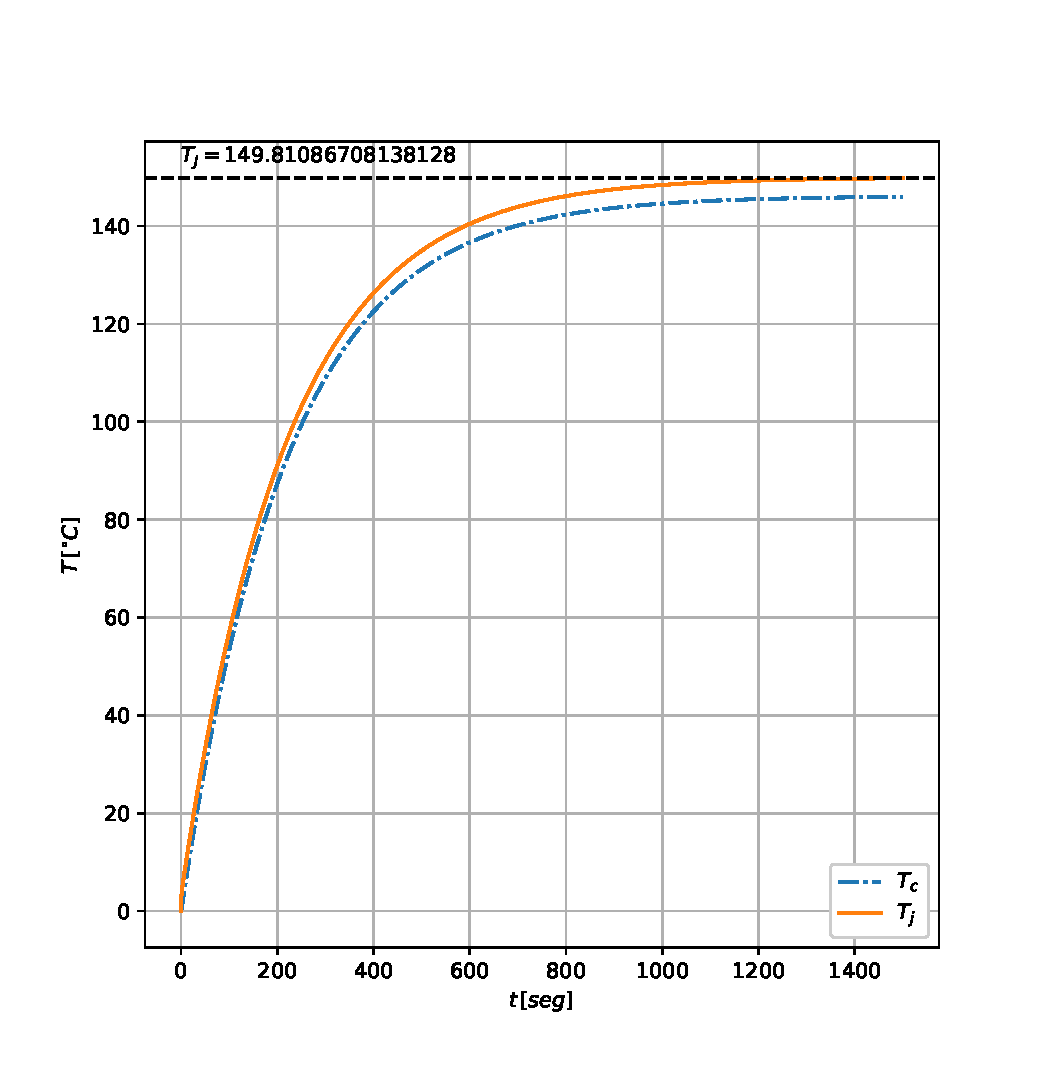
\includegraphics[width=0.50\linewidth]{Images/sin_disipador_step.eps}}
   \subfloat[]{\label{fig:sin_disipador_pulse}
   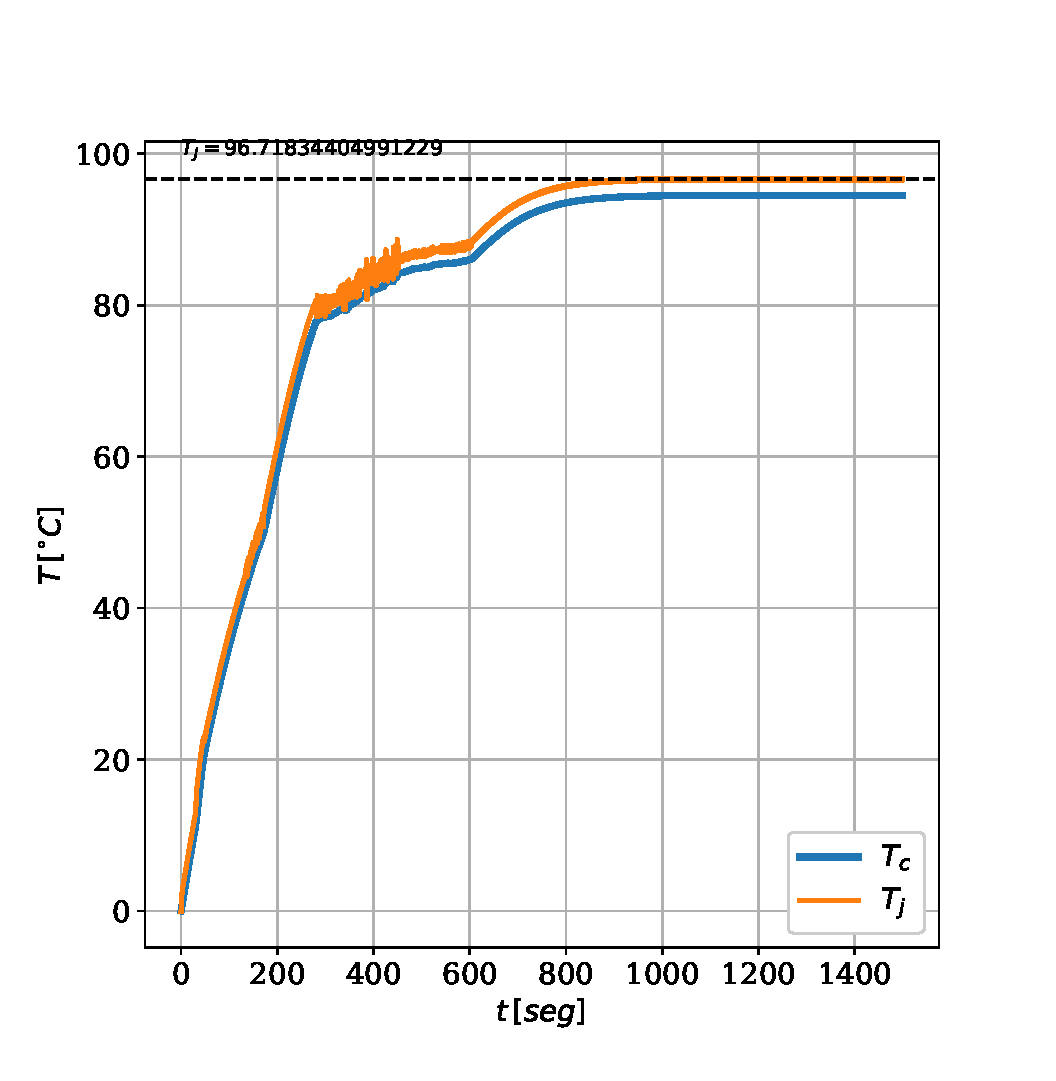
\includegraphics[width=0.50\linewidth]{Images/sin_disipador_pulse.eps}}%[20pt]
   \caption{Respuesta del sistema sin disipador: (a) entrada: escalón (b) entrada: pulsante}
\end{figure}
%------------------------------------------------------------------------------
%                      fin problema 1
%------------------------------------------------------------------------------
%------------------------------------------------------------------------------
%                      problema 2
%------------------------------------------------------------------------------
\section{Modelado y simulación de un sistema de calentamiento solar}
\begin{enumerate}
   \item Modele matemáticamente el sistema de calentamiento, tomando como variable de salida la temperatura $\theta(t)$
   \item Halle el flujo de calor por radiación necesario para obtener en estado estacionario una temperatura de salida $\theta_{ref}=60^{\circ}C$
   \item Obtenga el tiempo necesario para alcanzar dicha temperatura, si el fluido a calentar se encuentra a $\theta_{0}=15^{\circ}C$
   \item En época invernal la radiación solar se reduce notablemente y es insuficiente para alcanzar la temperatura deseada. Considere una situación en donde la
      radiación es del $40\%$ de la obtenida en el item anterior, y la temperatura inicial del fluído es de $15^{\circ}C$. Cual es la temperatura de estado
      estacionario en estas condiciones?
   \item Diseñe un circuito que complemente el colector solar para lograr la temperatura deseada de $60^{\circ}C$. Cuando el sistema de calentamiento se encuentra
      funcionando en lazo abierto, cualquier pequeña perturbacion en las condiciones teóricas de operación produce una desviación no deseada en la temperatura
      estacionaria de salida. Por este motivo, se ha introducido un controlador PI para garantizar el seguimiento de la consigna de temperatura en estado estacionario.
      De esta manera, una vez cerrado el lazo, la potencia calorífica que se suministra al circuito complementario es calculada directamente por el algoritmo de
      control y la nueva variable de entrada al sistema es entonces la temperatura de referencia $\theta_{ref}$
   \item Modele matemáticamente el sistema a lazo cerrado, tomando como variable de salida la temperatura $\theta(t)$ y como variable de entrada su valor de referencia $\theta_{ref}$
   \item Simule la evolución dinámica de la temperatura del sistema desde un instante inicial $\theta_{0}$ hasta un valor de referencia $\theta_{ref}$, operando
      en lazo abierto y en lazo cerrado, para tres valores distintos de ambas temperaturas.
   \item Estudie el comportamiento del sistema a lazo abierto y a lazo cerrado frente a perturbaciones de tipo escalón y rampa en la variable de entrada.¿Qué
      conclusión extrae de la eficiencia del controlador PI en ambos casos?¿Que sucedería si se utiliza sólo acción proporcional?
\end{enumerate}

\begin{figure}[H]
   \centering
   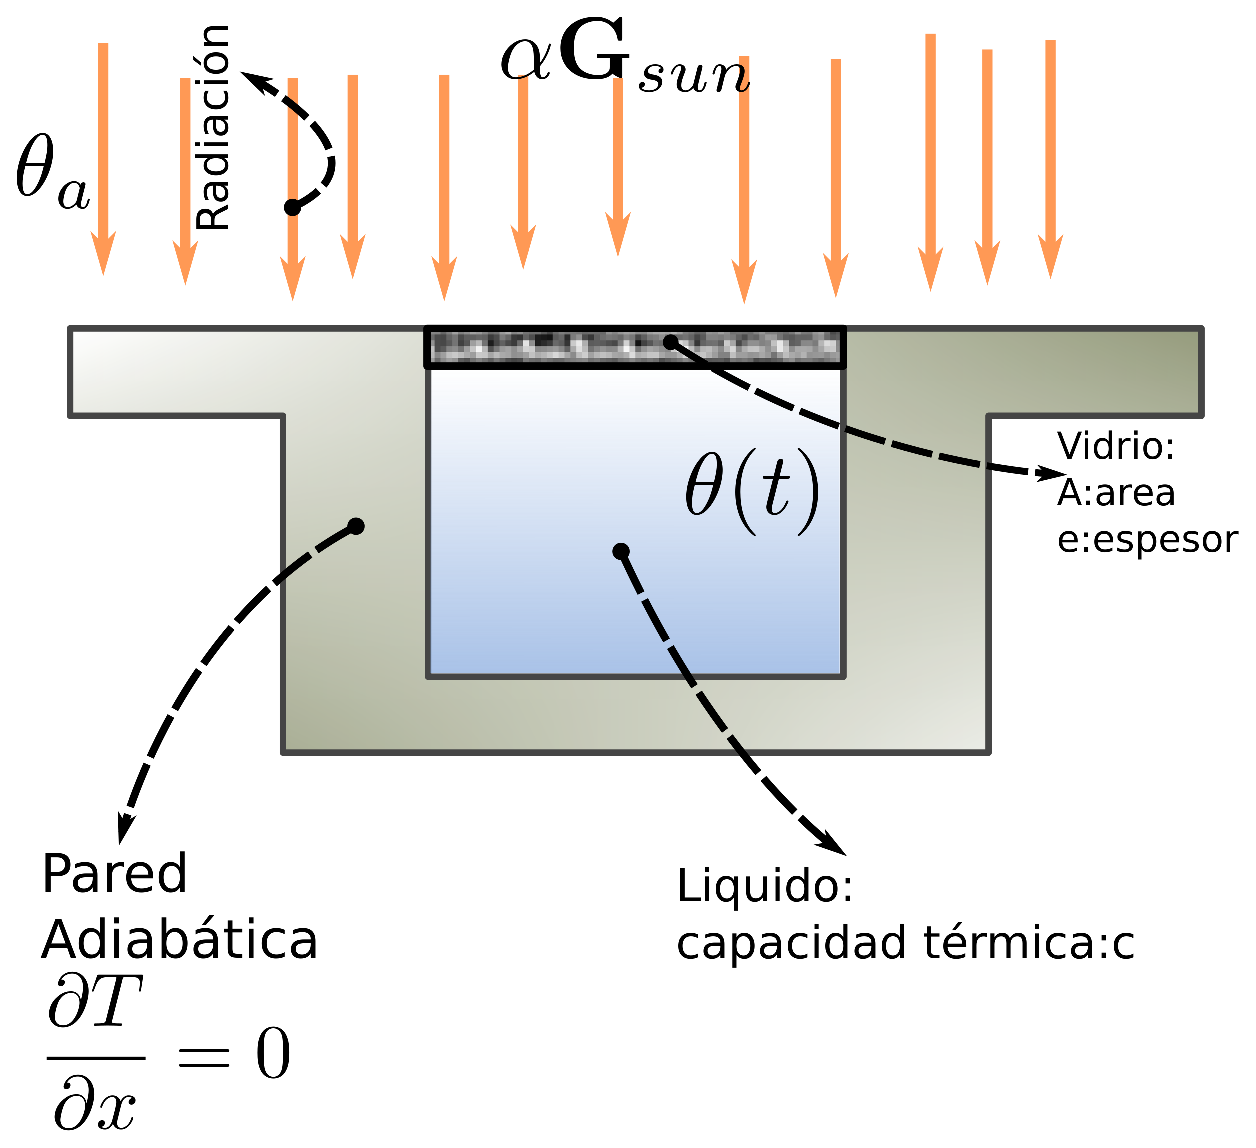
\includegraphics[width=0.37\textwidth]{Images/colector_esquema.eps}
   \caption{Esquema del colector solar}\label{fig:colector_esquema}
\end{figure}
%------------------------------------------------------------------------------
%                      fin problema 2
%------------------------------------------------------------------------------

%------------------------------------------------------------------------------
%                      problema 3
%------------------------------------------------------------------------------
\section{Modelado y simulación de un sistema de almacenamiento y distribución de agua}
En la figura se muestra de almacenamiento y distribución de agua en una vivienda unifamiliar promedio. El tanque tiene una capacidad de $1.5\,m^{3}$ y esta instalado
al nivel del piso. La \textit{bomba I} debe garantizar una carga completa del tanque en media hora. En regimen de trabajo, el tanque se debe mantener en los niveles
especificado en la figura. Ademas, la \textit{bomba II} se utiliza para mantener la presion constante en la vivienda. Para estas condiciones de trabajo:
\begin{enumerate}
   \item Elija bombas comerciales que puedan utilizarse en este problema. Justificar eleccion utilizando simulaciones, datos de funcionamiento y/o costo de las bombas.
   \item Desarrolle un control para cada bomba y simular el funcionamiento del sistema en regimen de trabajo.
   \item Cuales son los equipos de presurizacion existentes en el mercado. Cual eligiria para este proyecto. Justifique
\end{enumerate}
%------------------------------------------------------------------------------
%                      fin problema 3
%------------------------------------------------------------------------------
%-------------------------------------------------------------------------
% Bibliografia
%-------------------------------------------------------------------------
\begin{thebibliography}{6}
   \bibitem{Principal}{Incropera y De Witt, \textit{Fundamentos de transferencia de calor}, 4Ed}
\end{thebibliography}

\end{document}
